\section{Experiments}
\label{sec:experiments}

We validate the approach on ImageNet and CIFAR-10. We first describe the experimental and evaluation
set-up for both datasets and then present results under several scenarios.

\subsection{Set-up}
\textbf{ImageNet} We fix about 64,000 images for which
we have labels available (supervised set, $\mathcal{S}$). We use an additional 200,000 images as the
unsupervised set, $\mathcal{U}$. We use the ImageNet validation set for testing. It has 50,000
images spread over all 1,000 classes. We train DenseNet-161 networks scratch and report the
top-1 accuracy for all our experiments. Unless stated otherwise, we use a batch-size of 52 for all
ImageNet experiments. We later discuss that this might not be the ideal batch-size. However,
training with much larger batch-sizes requires vast amounts of time and resources.

% Need to report errors instead of accuracy for ImageNet too.

\textbf{CIFAR-10} Following prior work on semi-supervised learning, we use 4,000
images as the supervised set, and the other 46,000 images as the unsupervised set. Each setting
is repeated 5 times with the supervised set selected randomly each time. We test on the CIFAR-10
test set which contains 10,000 images spread over all 10 classes. The mean and standard
deviation of the errors are reported as the performance metric. We use the CIFAR-10 specific
DenseNet-121 network architecture. We use a batch-size of 64 for all CIFAR-10 experiments. 

We follow the training details from \cite{densenet} for training all networks. These include
the optimizer, momentum, and the learning rate schedule.

\subsection{Significance of Unsupervised Losses}
In this section, we show the utility of each unsupervised component of the loss in equation \ref{eq:total}. We
start with the baseline model where we use only the supervised images to train the network with only cross-entropy
loss. We progressively add more components to the optimization objective and report the
corresponding performance results and observations.

\subsubsection{Baseline}
As the baseline, we train a network using $\mathcal{S}$ as the training set and only $J_C$ as the
objective. Our DenseNet-161 model achieves a top-1 accuracy of $42.04\%$ on the ImageNet validation
set. 

For CIFAR-10, the baseline model reaches an error of $20.16\% \pm 1.02$. Comparing this to the $5.13\%$
error achieved by training the same network on the whole dataset, we note that the error rate is
very far from desired. We show that this gap can be reduced by using the available unsupervised data and
the proposed loss functions.  

\subsubsection{Cross-entropy + MEL}
Now, we add the $J_M$ term to the loss function, i.e., $\mathcal{L} = J_C + \alpha
J_M$ and use $\mathcal{S} \cup \mathcal{U}$ as the training set. We set $\alpha = 0.8$ and vary
$\frac{R}{T}$, i.e., the proportion of supervised images per batch. As $\frac{R}{T}$ increases, more
importance is given to the supervised data and loss components. Figure \ref{fig:acc} shows
the performance for ImageNet as we vary $\frac{R}{T}$ (top) and the variation in performance as we
increase the amount of unsupervised data used for a fixed $\frac{R}{T} = 0.7$ and a fixed supervised
set ($\mathcal{S}$) (bottom). 
% Need to remove the blue line from the curve or make it without dots. 
\begin{figure}
	\centering
	{
		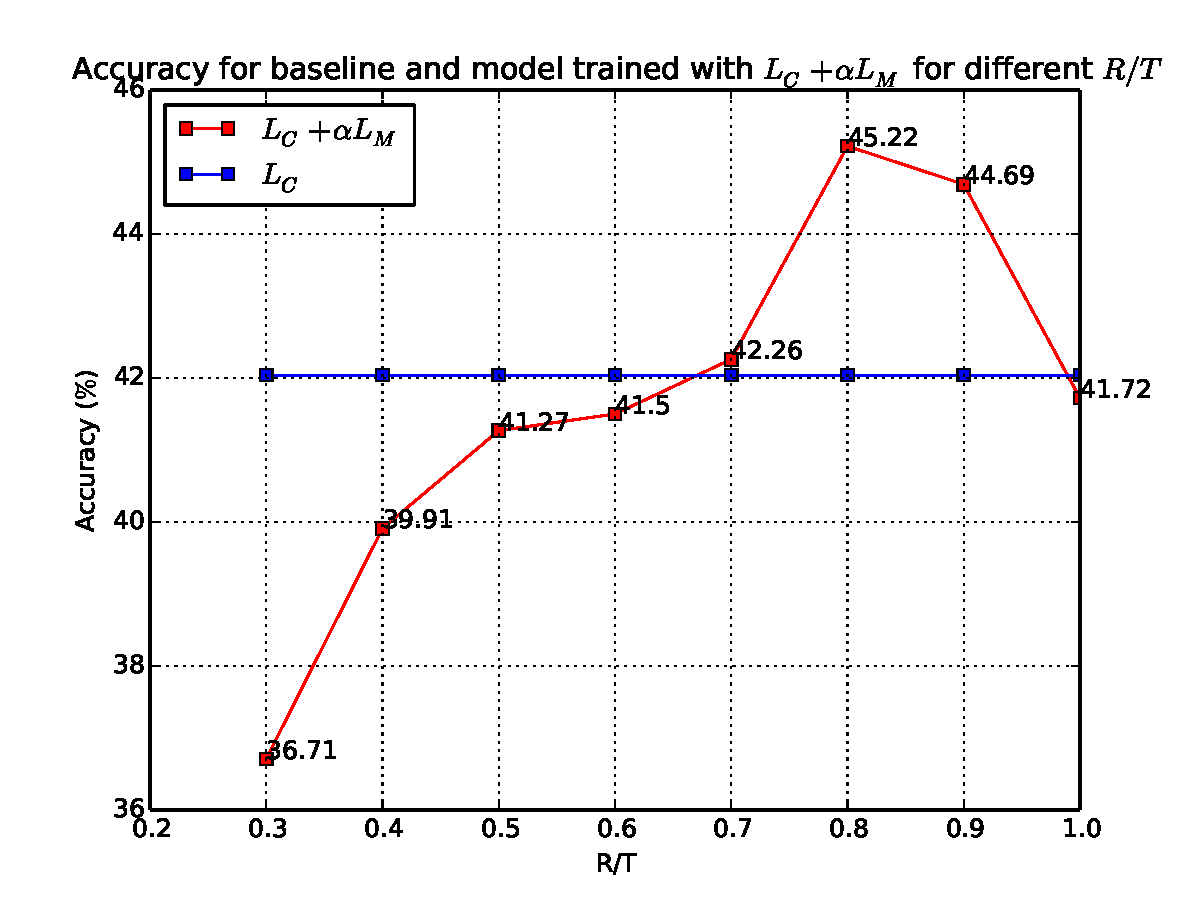
\includegraphics[scale=0.35]{accuracies.pdf}
	~
		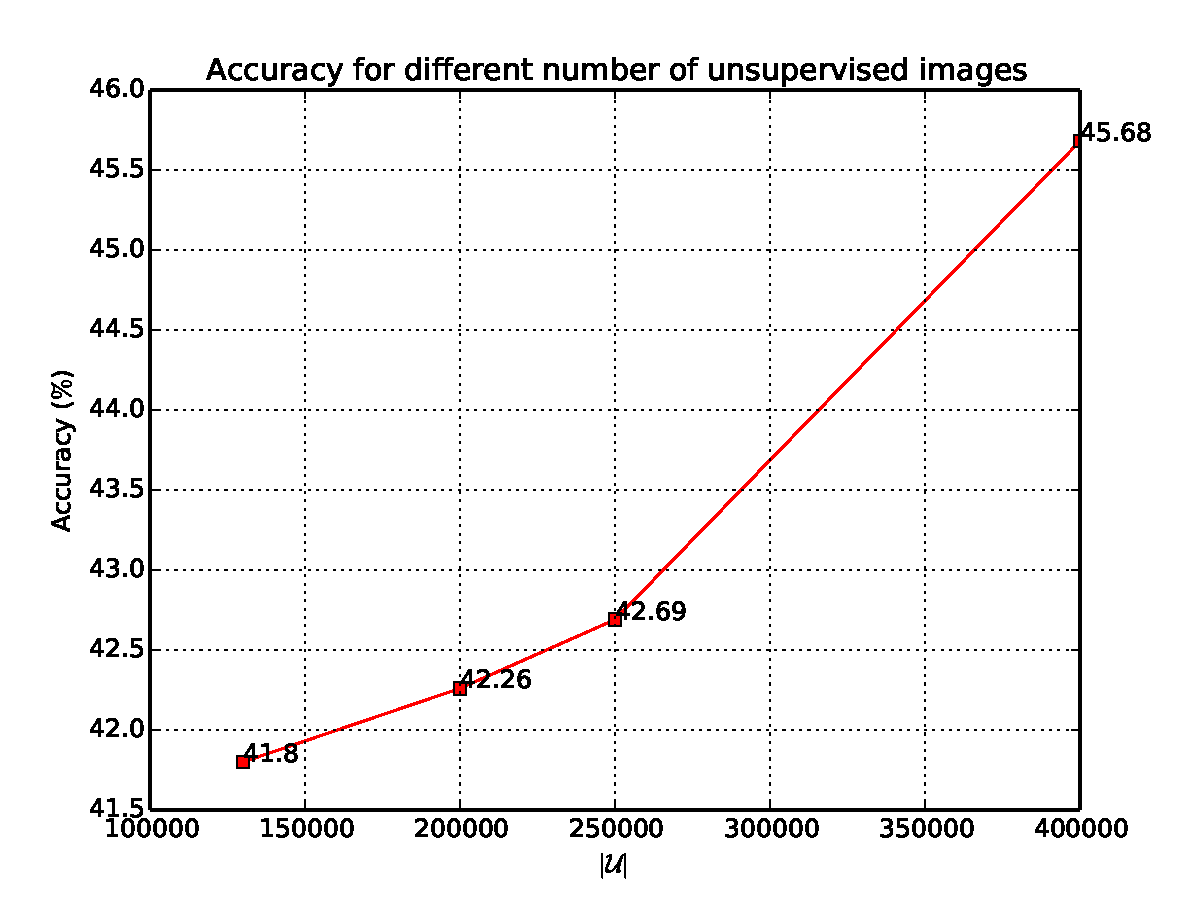
\includegraphics[scale=0.35]{accuracies_unsup.pdf}
	}
		\caption{(Top) Accuracy on the ImageNet validation set for models trained with the cross-entropy
		loss and MEL with $\mathcal{S}\cup\mathcal{U}$ (red). The blue line is the baseline
		performance and is here only for reference. (Bottom) Accuracy of models trained with
		cross-entropy loss and MEL with $\mathcal{S}\cup\mathcal{U}$ for $\frac{R}{T} = 0.7$ for
	different number of unsupervised images.}
		\label{fig:acc}
\end{figure}

Similarly, table \ref{tab:cifar_mel_ratio} gives the performance for CIFAR-10 as we vary the
supervision importance ratio $\frac{R}{T}$ and table \ref{tab:cifar_mel_unsup} shows how performance
varies as we vary the number of unsupervised images keeping the supervised set fixed. We see similar
trends in table \ref{tab:cifar_mel_unsup} as in figure \ref{fig:acc} (bottom). As we add more
unsupervised data with a fixed supervised set, the classification performance improves. This shows
that our method could be used to improve performance by using more unlabeled images in addition to
the supervised images during training.

\begin{table}
	\centering
	\begin{subtable}{0.15\textwidth}
	\centering
	\begin{tabular}{|c|c|}
		\hline
		a & b \\
		\hline
		c & d\\
		\hline
	\end{tabular}
	\caption{}
	\label{tab:cifar_mel_ratio}
	\end{subtable}
	%
	\begin{subtable}{0.15\textwidth}
	\centering
	\begin{tabular}{|c|c|}
		\hline
		a & b \\
		\hline
		c & d\\
		\hline
	\end{tabular}
	\caption{}
	\label{tab:cifar_mel_unsup}
	\end{subtable}
\end{table}

\subsubsection{Cross-entropy + MEL + NBEL}
Next we add the negative batch-entropy loss to cross-entropy loss and MEL. We vary $\beta$ while
keeping $\alpha$ and $\frac{R}{T}$ fixed from the previous case. The performance (accuracy on the
validation set) of these models hasn't reached the level of the previous cases. We
believe that this is because of the small batch sizes that we are using. Our next steps for this are
to increase the batch-size by using more GPUs or accumulating gradients over a few iterations before
updating the parameters.

\subsubsection{Cross-entropy + Loc}
In this case, we take the class activation map (CAM) of the class with the highest probability and
apply the locality penalty to this CAM. We have observed that CAMs
are able to localize some objects, but we haven't analyzed whether this is because of the
formulation of CAMs or because of our loss function. We plan to see the evolution of the
activations as training progresses to see if the area covered by the activations is reducing and
whether the CAMs are becoming more accurate with more training. 

\subsubsection{Data Efficiency}





\subsubsection{Transfer Learning}
%For a comparison with recent work on unsupervised learning, we will experiment
%with the transfer learning setting too. In this setting, models trained with only unsupervised
%losses are used as initializations for other tasks (e.g. object detection, semantic segmentation).
%We want to compare the unsupervised losses used by these works against ours. We also want to see if
%models trained with both supervised and unsupervised losses are better than models trained with only
%unsupervised losses for transfer learning. 


\subsection{Results}
We present results and comparisons.

\begin{table}
	\centering
	\begin{tabular}{|c|c|}
		\hline
		\textbf{Method} & \textbf{Error} \\
		\hline
		Ladder Net \cite{Rasmus2015} & \\
		\hline
		Temporal Ensembling \cite{Laine2016}  & \\
		\hline
		Regularization \cite{Sajjadi2016a}  & \\
		\hline
		CCL \cite{Kamnitsas2018}  & \\
		\hline
		Improved Techniques \cite{Salimans2016}  & \\
		\hline
		CatGAN \cite{Springenberg2015}  & \\
		\hline
		TripleGAN \cite{Li2017}  & \\
		\hline
		BadGAN \cite{Dai2017}  & \\
		\hline
		\hline
		Only $J_C$ (Ours)  & \\
		\hline
		$J_C + J_M$ (Ours)  & \\
		\hline
		$J_C + J_M + J_B$ (Ours)  & \\
		\hline
		$J_C + J_L$ (Ours)  & \\
		\hline
		$J_C + J_M + J_L$ (Ours)  & \\
		\hline
		$J_C + J_M + J_B + J_L$ (Ours)  & \\
		\hline
		$J_C + J_M + J_B + J_L$ (Ours) $+$  & \\
		Regularization  & \\
		\hline
	\end{tabular}
	\caption{CIFAR-10 Results}
	\label{tab:cifar_results}
\end{table}





\begin{table}
	\centering
	\begin{tabular}{|c|c|}
		\hline
		\textbf{Method} & \textbf{Error} \\
		\hline
		Regularization \cite{Sajjadi2016a}  & \\
		\hline
		\hline
		Only $J_C$ (Ours)  & \\
		\hline
		$J_C + J_M$ (Ours)  & \\
		\hline
		$J_C + J_M + J_B$ (Ours)  & \\
		\hline
		$J_C + J_L$ (Ours)  & \\
		\hline
		$J_C + J_M + J_L$ (Ours)  & \\
		\hline
		$J_C + J_M + J_B + J_L$ (Ours)  & \\
		\hline
		$J_C + J_M + J_B + J_L$ (Ours) $+$  & \\
		Regularization  & \\
		\hline
	\end{tabular}
	\caption{ImageNet Results}
	\label{tab:imagenet_results}
\end{table}

